% LISTA DE EXERCÍCIOS Template using "book"
% Created by Milena Lima 
%Email:milenascimentolima@gmail.com
% Science Project at school 2017-FAPEAM
% View: https://www.overleaf.com/read/syjxcffdygch
%=======================================================
%------------LISTA DE EXERCÍCIOS
%=======================================================
\documentclass[12pt,a4paper,oneside,openany]{book} 
%=======================================================
%-------------PACOTES 
%=======================================================
\usepackage[top=1cm,left=1cm,right=1.5cm,bottom=2cm]{geometry}
\usepackage[T1]{fontenc}%Especif. a codif. de caracteres
\usepackage{ae}%Auxílio para fontes e pdf
\usepackage[utf8]{inputenc}
\usepackage{lipsum}%Gerar Texto Aleatório
\usepackage{babel}%Traduzir para Português
\usepackage{indentfirst}%Faz indentações em parágrafos
\usepackage{graphicx}%Permite incluir figuras
\usepackage{subfig} %para criar sub figuras
\usepackage{float}% figuras
\usepackage{tabularx}
\usepackage{ragged2e}
\usepackage{multirow}
\usepackage[dvipsnames]{xcolor}%Admitir cores
\usepackage{amsmath,amssymb,amsthm}%Incluir expressões  matemáticas, equações, teoremas, símbolos, etc
\usepackage{lastpage}%Incluir Ficha catalográfica
\usepackage{epigraph}%Incluir Epígrafo
\usepackage{enumerate}
\usepackage{enumitem}
\usepackage{listings}
\newlist{questions}{enumerate}{3}
\setlist[questions]{label=\arabic*.}
\newcommand{\question}{\item}
\setlist[enumerate,1]{% (
leftmargin=*, itemsep=12pt, label={\textbf{\arabic*.)}}}
%---
\newlist{partes}{enumerate}{3}
\setlist[partes]{label=(\alph*)}
\newcommand{\parte}{\item}
%---
\newlist{subpartes}{enumerate}{3}
\setlist[subpartes]{label=\roman*)}
\newcommand{\subparte}{\item}
%---
\usepackage{array}
\usepackage{tikz}
\newcommand*\circled[1]{\tikz[baseline=(char.base)]{\node[shape=circle,draw,inner sep=2pt] (char) {#1};}}
\usepackage[sort&compress,round,comma,authoryear]{natbib}
\usepackage{makeidx}
\PassOptionsToPackage{hyphens}{url}
\usepackage[colorlinks=true,urlcolor=magenta,citecolor=red,linkcolor=violet,bookmarks=true]{hyperref}
\usepackage{lscape}%Altera a orientação de uma página
\usepackage{pdflscape}
\usepackage{epstopdf} %converte figs eps em figs pdf
\usepackage{booktabs}
\usepackage{pdfpages}
\usepackage{textcomp}
\usepackage[many]{tcolorbox}
\usepackage{empheq}
\usepackage{tasks}%lista alfabética
\pagestyle{plain}
\renewcommand{\ttdefault}{pcr}
%================================================================
%------------DIGITE AQUI
%===============================================================
\newcommand{\orgao}{University of St.Gallen}
\newcommand{\instituto}{Institute of Computer Science}
\newcommand{\curso}{Einführung in Computersysteme, HS2026}
\newcommand{\professor}{Luka Bekavac, Karim Khamaisi, Simon Mayer}
\newcommand{\titulo}{Assignment 1: Bare Metal Raspberry Pi Setup (10pt)\\\small{Deadline: October 11th, 2026; 23:59 CET}}
\newcommand{\data}{\today}
\newcommand{\email}{\{luka.bekavac, karim.khamaisi, simon.mayer\}@unisg.ch}
\newcommand{\repo}{https://github.com/Interactions-HSG/2026-HS-ICS-Assignment1}
%===========================================================
\newcommand{\X}{\mathbf{X}}
\newcommand{\x}{\mathbf{x}}
\newcommand{\Z}{\mathbf{Z}}
\newcommand{\z}{\mathbf{z}}
\newcommand{\y}{\boldsymbol{y}}
\newcommand{\balpha}{\mbox{${ \bm \alpha}$}}
\newcommand{\bmu}{\mbox{${\bm \mu}$}}
\newcommand{\bbeta}{\mbox{${\bm \beta}$}}
\newcommand{\bteta}{\mbox{${\bm \theta}$}}
\newcommand{\bgama}{\mbox{${\bm \gamma}$}}
\newcommand{\bxi}{\mbox{${\bm \xl}$}}
\newcommand{\bvarphi}{\mbox{${ \bm \varphi}$}}
\newcommand{\SZ}{\mbox{ $Z$}}
\newcommand{\muz}{\mu_{z,l}}
\newcommand{\muo}{\mu_{0,l}}
\newcommand{\etao}{\eta_{0,l}}
\newcommand{\etaz}{\eta_{z,l}}
\newcommand{\xbeta}{x_{l}\bgama}
\newcommand{\mui}{\mu_{l}}
\newcommand{\zetaind}{\zeta \mathtt{I}_{\{s_{l} \in Z \}}} 
\newcommand{\spz}{ s_{l} \in z}
\newcommand{\snpz}{ s_{l} \notin z}
\newcommand{\sps}{ s_{l} \in S}
\newcommand{\gphi}{ \Gamma(\phi)}
\newcommand{\scan}{ \Lambda_{z}}
\newcommand{\gmuop}{ \Gamma(\muo\phi)}
\newcommand{\gmuzp}{ \Gamma(\muz \phi)}
\newcommand{\gumuop}{ \Gamma((1-\muo)\phi)}
\newcommand{\gumuzp}{ \Gamma((1-\muz)\phi)}
\newcommand{\dlobeta}{ \frac{\parteial l_{0}(\bgama, \phi, 0) }{\parteial \bgama}}
\newcommand{\lz}{  l_{z}(\bgama, \phi, \tau)}
\newcommand{\lo}{  l_{0}(\beta, \phi, 0)}
\newcommand{\E}{\mathbb{E}}
\newcommand{\dis}{\displaystyle}
\linespread{1.0}%espaço entre linhas
\begin{document}

\definecolor{mygray}{rgb}{0.9,0.9,0.9}

\lstset{ %
	language=C,
    backgroundcolor=\color{mygray}
}

%%%%%%%%%%%%%%%%%%%%%%%%%%%%%%%%%%%%%%%%%%%%%%%%%%%%%%%%
%                      CABEÇALHO                     %
%%%%%%%%%%%%%%%%%%%%%%%%%%%%%%%%%%%%%%%%%%%%%%%%%%%%%%%%
\begin{table}[H]
\centering
\begin{tabular*}{\textwidth}{l@{\extracolsep{\fill}}l@{\extracolsep{\fill}}}
\begin{tabular}[l]{@{}l@{}}\textbf{\orgao}\\\\\textbf{\instituto}\end{tabular} & \begin{tabular}[l]{@{}l@{}}\textbf{\curso}\\\professor \\{\email}\end{tabular}                                                       
\end{tabular*}
\end{table}
\begin{center}
\rule[2ex]{\textwidth}{1pt}\\
{\Large{\titulo}}
\end{center}
\rule[2ex]{\textwidth}{1pt}\\

In this assignment, you will set up your local programming environment for ``bare metal'' development on the Raspberry Pi platform and create, compile, and run a few simple programs on the hardware. To solve the assignment, you need a \textit{Raspberry Pi 400 PC-Kit}, a \textit{330$\Omega$ resistor}, an \textit{LED}, a \textit{Breadboard}, and two \textit{Male-to-Female jumper wires}. 

\textbf{Everything you need is in the assignment repository:}
\begin{center}
\url{\repo}
\end{center}

\noindent Start by reading the \texttt{README.md} there -- it walks you through creating your own copy, step by step, and assumes you have never used Git before.

You work in your \textbf{assigned group of two} and share \textbf{one} repository: one of you creates it from the template, the other joins as a collaborator.

By the deadline, you hand in that \textbf{GitHub repository}. There is no zip file, and only \textbf{one of you} submits -- on Canvas you hand in \textbf{only the URL of your repository}. It must contain:

\begin{itemize}
    \item \textbf{Tasks 1, 2, 3 and 5:} Your answers in the file \texttt{REPORT.md}. All questions below are already written out in that file -- you only fill in the blanks. Please also state there your \textbf{group number}, the names of \textbf{both} team members and their roles, the major pitfalls you encountered, and how many minutes/hours you spent on this assignment.

    \item \textbf{Task 2:} A screenshot named \texttt{screenshots/t1.png} of your console window showing the version of your \texttt{arm-none-eabi-objcopy} command.

    \item \textbf{Task 4:} Your code in the file \texttt{led\_blink.c}

    \item \textbf{Bonus Task:} Your code in the file \texttt{led\_fade.c}
\end{itemize}

\noindent Three things we cannot grade without, so please do not forget them:
\begin{itemize}
    \item Your repository must be \textbf{private} -- use the \textbf{Use this template} button on the page above, \textbf{do not fork}.
    \item It must be named \texttt{\textbf{ics-a1-group<your number>}}, using your group number from Canvas, digits only -- for example \texttt{\textbf{ics-a1-group7}}. We match repositories to groups by that name.
    \item You must add \textbf{your partner}, \texttt{\textbf{lukabekavac}} and \texttt{\textbf{Karimkh31}} as \textbf{collaborators} on your repository.
\end{itemize}

\vspace{10mm}

\begin{center}

\textbf{We wish you a lot of fun with your first (?) embedded computing project!}
\end{center}

\vspace{10mm}

\textbf{On using AI:} you are encouraged to use AI tools for this assignment. But do not ask ``solve this for me'' -- ask ``explain how to solve this''. The point of this assignment is that you end up able to read a hardware manual and reason about registers yourself. Note down in \texttt{REPORT.md} which tools you used and what for.

This assignment generally follows a tutorial on valvers.com\footnote{\url{https://www.valvers.com/open-software/raspberry-pi/bare-metal-programming-in-c-part-1/}}, however with a few twists:

\begin{itemize}
    \item You do \textbf{not} need to work on the \textit{Generating SD Cards} part of the tutorial, as we provide the relevant files for your SD card to enable you to focus on the essence of this assignment.
    \item For the same reason, the repository contains a file \texttt{power\_blink.c} that is derived from the \texttt{armc-03.c} file in the tutorial -- this file is specific to our version of the Raspberry Pi and thus simpler and easier to understand.
    \item The tutorial does not solve the assignment for you -- it merely presents you with a solution to a \textit{similar} problem that you will need to adapt to fit your needs.
    \item See \texttt{README.md} in the repository to get started, and \texttt{docs/TOOLCHAIN.md} for the exact commands you will need.
\end{itemize}

\newpage

\begin{questions}[label=\protect\circled{\bfseries\arabic*}]

\question \textbf{Bandit Game: level 3 - 10 (1pt)}

In this task, you are asked to work through the \textbf{OverTheWire Bandit}\footnote{\url{https://overthewire.org/wargames/bandit/bandit4.html}} challenges from  \emph{Level 3 -> Level 4} up to \emph{Level 9 -> Level 10}.

You are asked to document both the \textit{steps} and the \textit{passwords} you found. For each level, write down:
\begin{itemize}
   \item The command(s) you used
   \item The password you discovered
   \item How you found the solution
\end{itemize}

\textbf{One-Liner Challenge:} As an additional challenge, you are encouraged to combine multiple commands into a single line using pipes (\texttt{|}) and command chaining (\texttt{\&\&}, \texttt{;}) wherever possible. If a solution requires multiple commands, try to chain them into one efficient command.

\question \textbf{Toolchain Setup (1pt)}

In this task, you set up and test your toolchain for compiling bare metal programs and deploying them onto your Raspberry Pi.

%\begin{partes} \parte
\textbf{Setting up your Programming \& Compilation Environment}

Set up a GCC ARM compilation environment on your machine (available for Linux, Windows and Mac from here\footnote{\url{https://developer.arm.com/downloads/-/arm-gnu-toolchain-downloads}}), where we will be working with the \texttt{arm-none-eabi-xx} toolchain for 32bit systems (i.e. \textit{ARM processor / NO operating system / embedded Application Binary Interface}). Install this toolchain (version 13.3.Rel1);
% after installing the toolchain, add the \texttt{bin} directory of the installed software to your system's PATH (see below).

\begin{itemize}
    \item For Windows: Download and use \\
    \texttt{arm-gnu-toolchain-13.3.rel1-mingw-w64-i686-arm-none-eabi.exe}. You can add the installation directory to the \texttt{PATH} environment variable at the end of the installation wizard (See Figure ~\ref{fig:gnutool}).
    
    \item For Mac: Download and use \\
    \texttt{arm-gnu-toolchain-13.3.rel1-darwin-x86\_64-arm-none-eabi.pkg} \\
    or \texttt{arm-gnu-toolchain-13.3.rel1-darwin-arm64-arm-none-eabi.pkg} for Apple silicon (You can check the processor in system information).
    % See the \texttt{README.md} file to find how to appropriately set the \texttt{PATH} environment variable.
\end{itemize}

\begin{figure}[ht]
        \centering
        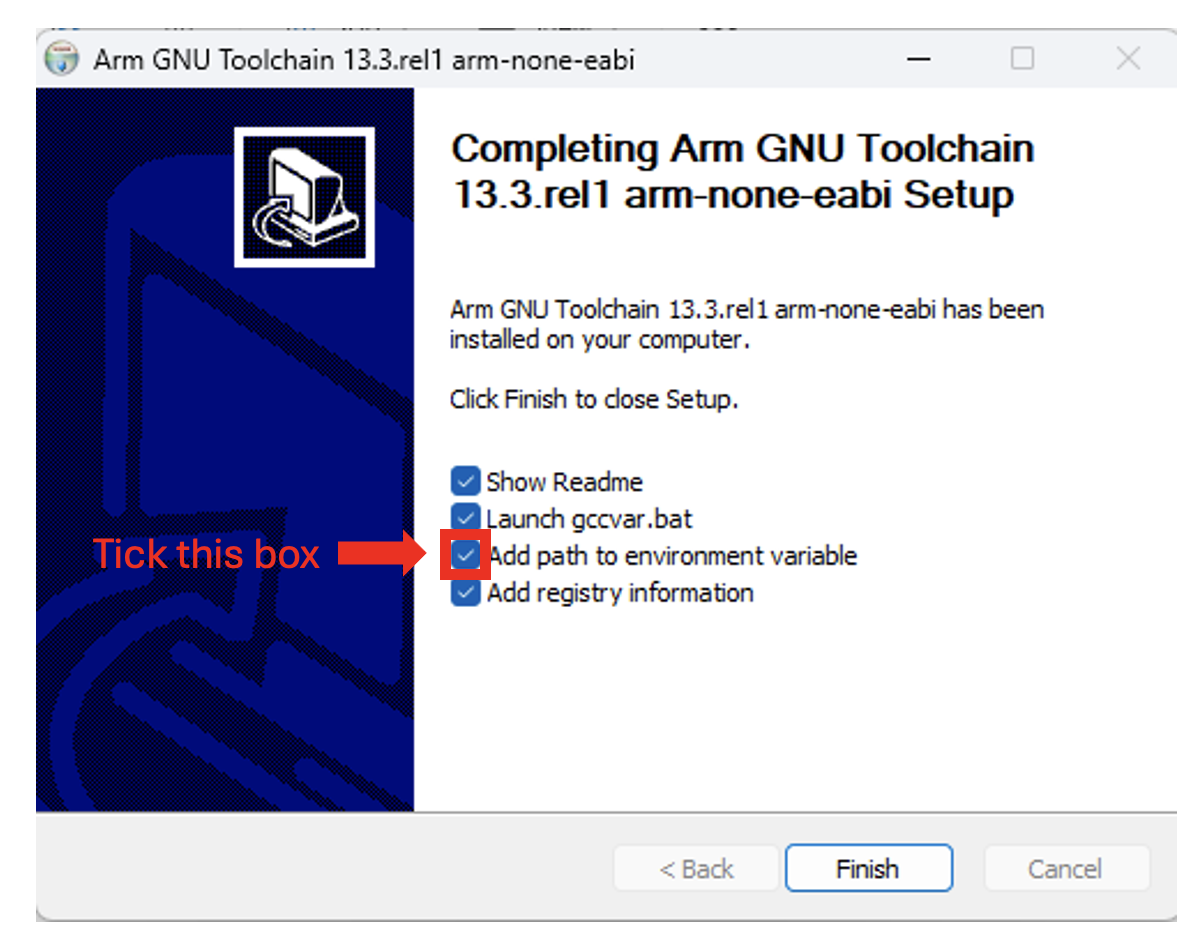
\includegraphics[width=.5\linewidth]{figures/gnutool.png}
        \caption{The GNU Toolchain installation wizard.}
        \label{fig:gnutool}
\end{figure}
    
% Finally, make sure that the commands \texttt{arm-none-eabi-gcc} (with the installed gcc version) and \texttt{arm-none-eabi-objcopy} work as expected from a console window (i.e., ``PowerShell'' in Windows and ``Terminal'' in Mac).


Add the path to the toolchain bin directory to the environment variable `\$PATH`

On MacOS, the executable binaries are installed at \texttt{/Applications/ArmGNUToolchain/\{your toolchain version\}/arm-none-eabi/bin}. To add this to your PATH environment variable, use the command given in \texttt{docs/TOOLCHAIN.md}. This command appends a single line at the end of your ZSH (the default shell on MacOS) user configuration file.

If the toolchain is successfully installed, you should see something like Figure \ref{fig:gcc} when typing \texttt{arm-none-eabi-gcc -{}-version[ENTER]} in Mac Terminal or \texttt{arm-none-eabi-gcc-13.3.1.exe -{}-version} in Windows PowerShell; also see \texttt{docs/TOOLCHAIN.md} for this.


\begin{figure}[ht]
  \centering
    \subfloat[{In MacOS Terminal}\label{fig:gcc-mac}]{%
    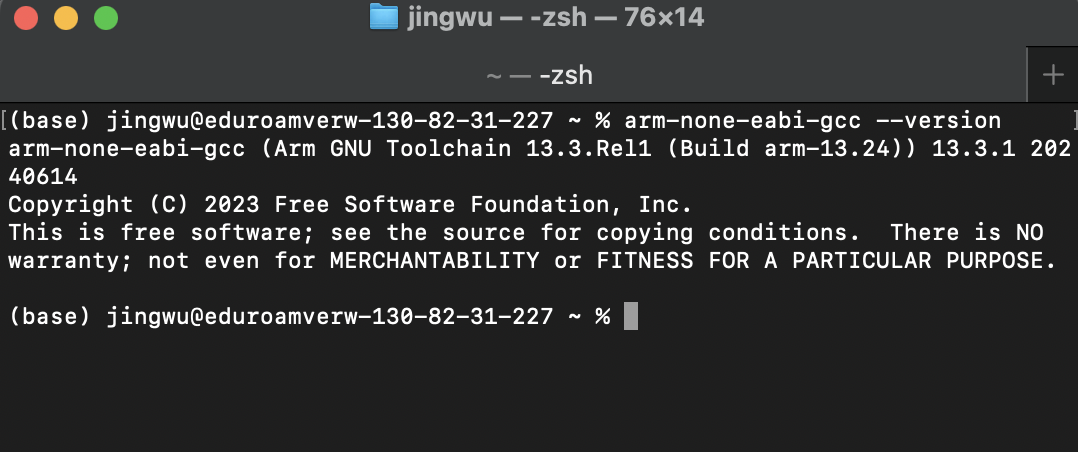
\includegraphics[width=.6\linewidth,keepaspectratio]{figures/gcc-mac.png}}
    \hfill
  \subfloat[{In Windows PowerShell}\label{fig:gcc-win}]{%
    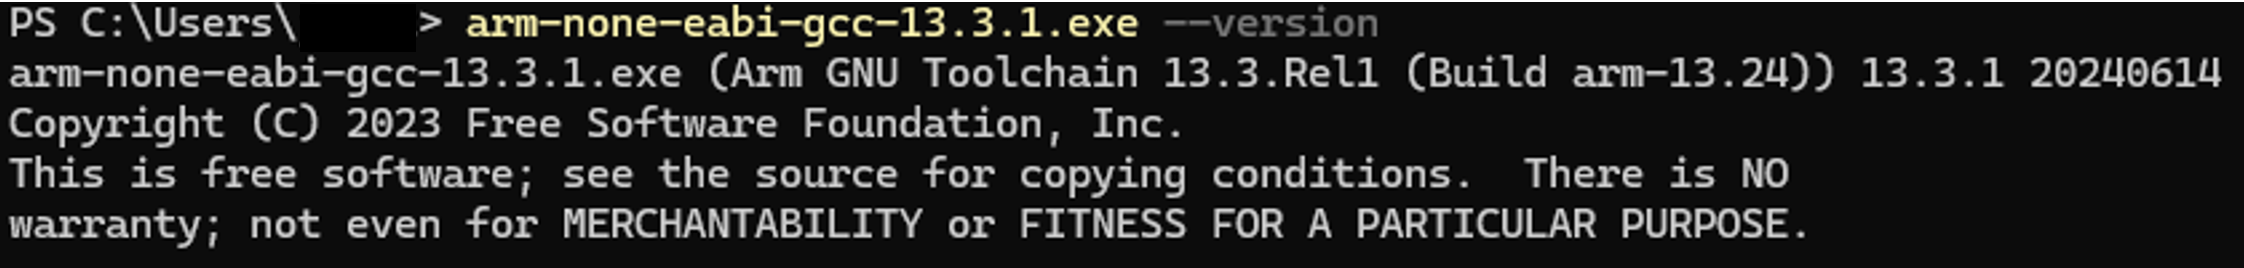
\includegraphics[width=.9\linewidth,keepaspectratio]{figures/powershell-gcc-version.png}}
    \hfill
  \caption{Show the installed version of \texttt{arm-none-eabi-gcc}.}
  \label{fig:gcc}
\end{figure}


\question \textbf{Bare Metal ``Hello World'' (4pt)}

In this task, you compile and deploy a simple program that will blink your Raspberry Pi's power LED -- a classic ``Hello World'' program for embedded computing.

\begin{partes}

\parte \textbf{Prepare the SD card (0.5pt)}

Format the SD card in \textbf{FAT32} file system\footnote{Find instructions online.} so that the RPi can use your custom kernel image to boot up with. The SD card also needs to contain specific files. Copy the 3 files (\texttt{config.txt}, \texttt{fixup4.dat}, and \texttt{start4.elf}) that you find in the \texttt{boot/} directory in your repository onto the formatted SD card -- do not create a \texttt{boot/} directory on the SD card, just copy the files.

Raspberry Pi 400 uses an EEPROM to boot the system\footnote{\url{https://www.raspberrypi.com/documentation/computers/raspberry-pi.html\#raspberry-pi-4-boot-eeprom}}.
The bootloader can be configured using the file \texttt{config.txt}\footnote{\url{https://www.raspberrypi.com/documentation/computers/config_txt.html\#boot-options}} and therefore a minimal firmware is provided in \texttt{fixup4.dat} and \texttt{start4.elf}.
For the Raspberry Pi 400, the default filename on the boot partition to use when loading the kernel is \texttt{kernel7l.img}\footnote{\url{https://www.raspberrypi.com/documentation/computers/config_txt.html\#kernel}}.

\parte \textbf{Blink the power LED (0.5pt)}

Using the toolchain from Task 2, ``cross-compile'' the code to be executed on the Raspberry Pi 400's Broadcom chip, the BCM2711\footnote{\url{https://www.raspberrypi.com/documentation/computers/processors.html\#bcm2711}}.
Follow the instructions in \texttt{docs/TOOLCHAIN.md} to produce a \texttt{kernel7l.img} file (or simply run \texttt{make power\_blink}) and copy this binary kernel image to the SD card. % (or simply use the provided \texttt{Makefile}\footnote{https://opensource.com/article/18/8/what-how-makefile}) and then copy the file to the SD card.
Eject the SD card from your computer, insert it into the Raspberry Pi, and connect the power adapter. The Raspberry Pi's Power LED should be blinking now.

\parte \textbf{Examine the code and understand the BCM2711 (3pt)}

Examine the code in \texttt{power\_blink.c}, together with the manual of the BCM2711 ARM Peripherals\footnote{\url{https://datasheets.raspberrypi.com/bcm2711/bcm2711-peripherals.pdf} (also provided in \texttt{docs/} in the repository)} -- particularly interesting for this assignment are pages 65-70 of the manual, as well as pages 4-6. Answer the following questions in \texttt{REPORT.md}:

\begin{enumerate}
    \item In line 51 of \texttt{power\_blink.c}, what is the register address represented by \texttt{\textbf{gpio[GPFSEL4]}} according to the manual? Provide your answer as an offset from the GPIO base address.
    
    \item Calculate the value \texttt{\textbf{(1 <{}< 6)}} and answer in binary notation. According to the manual, what does it mean when this value is written to the address \texttt{gpio[GPFSEL4]}?
    
    \item How would you modify this line in order to turn all the GPIO pins that are covered by the \textbf{GPIO Alternate Function Select Register 1} (i.e., GPIO 10-19) into \textbf{outputs}? (HINT: Use \texttt{0} for the reserved bit values.)
\end{enumerate}

\end{partes}

At this point, you should understand what this program does and why it works.


\question \textbf{Building your own Digital Circuit and Blinking an LED (4pt)}

Use your cables, resistors and breadboard to properly connect an LED to your Raspberry Pi 400 at \textbf{GPIO 16}\footnote{\url{https://pinout.xyz/}} (= The Pin 36) as shown in Figure \ref{fig:wiring}.

\begin{figure}[ht]
  \centering
  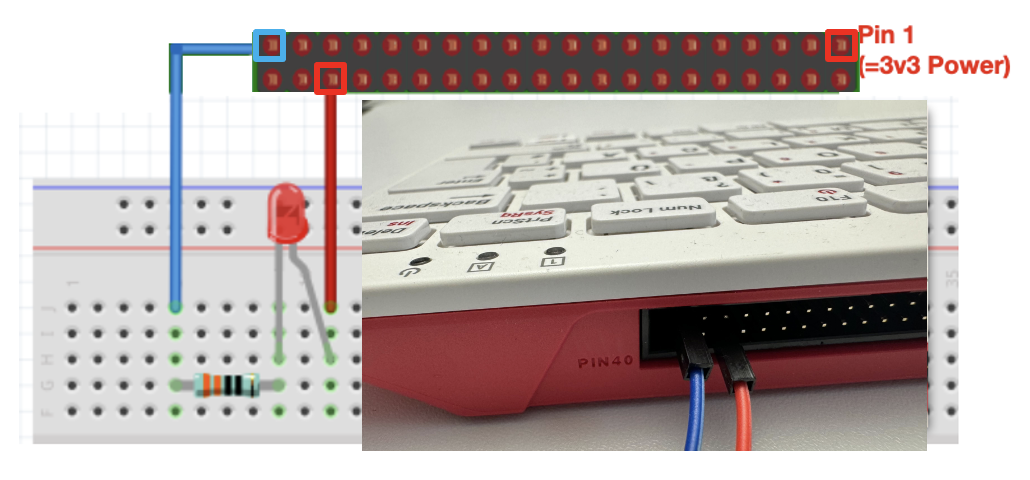
\includegraphics[width=.8\linewidth]{figures/wiring.png}
  \caption{The wiring diagram.}
  \label{fig:wiring}
\end{figure}

Your repository already contains \texttt{led\_blink.c}, which starts out as a copy of \texttt{power\_blink.c}. Modify it so that it blinks the \textit{external} LED that you connected to GPIO 16 instead of the Raspberry Pi's power LED. Build it with \texttt{make led\_blink}.
To solve this puzzle, you will need to consider again the BCM2711 manual.


\question \textbf{BONUS: LED Experiments (2pt)}

Extend your program in the file \texttt{led\_fade.c} (also already in your repository) with functionality that fades the LED in and out slowly instead of just turning it on/off.
There are multiple options of how this can be accomplished -- any functionally correct way will be accepted as a solution to this task!


\end{questions}


%================================================================
%-------------------FIM DA LISTA
%================================================================
%===========================================================
%          BIBLIOGRAFIA
%===========================================================
%\begin{thebibliography}{99}
%\thispagestyle{empty}%myheadings
%===========================================================
%==============Livro
%\bibitem[Hazzan(1993)]{Hazzan(1993)}
%[1] {Hazzan, Samuel}.
%\emph{Combinatória e Probabilidade}.
%{Volume  5}, {1;ed}, {São Paulo}, {Atual}, {1993}.
%===========================================================
%\end{thebibliography}
\end{document}